\documentclass{beamer}
\usepackage[utf8]{inputenc}
\usepackage[T1]{fontenc}
\usepackage{graphicx}
\usepackage{tcolorbox}
\usepackage{hyperref}
\hypersetup{
    colorlinks=true,
    linkcolor=pink,
    urlcolor=cyan,
    urlbordercolor=cyan,
}
\graphicspath{ {./images/} }
\newcommand\tab[1][0.3cm]{\hspace*{#1}}

\usetheme{Arguelles}

\title{Tutorial 4}
\subtitle{CS3241 Computer Graphics (AY22/23)}
\date{\today}
\author{Wong Pei Xian}
\institute[]{\email{e0389023@u.nus.edu}}

\begin{document}

\frame[plain]{\titlepage}

\section{Lecture 5}

\begin{frame}[plain,standout]
    \AlegreyaExtraBold \LARGE
    Lecture 5 (pg 48 to 49)
\end{frame}

\begin{frame}
    \frametitle{Recap}

    Lecture 4:
    \begin{itemize}
        \item Matrices (translation, rotation, scale)
        \item Matrix stacks (Current Transformation Matrix or CTM)
    \end{itemize}

    \vspace{1em}

    Lecture 5:
    \begin{itemize}
        \item View transformation
        \item Projection
        \item \texttt{GL\_MODELVIEW} and \texttt{GL\_PROJECTION} in context of CTM
    \end{itemize}

\end{frame}

\begin{frame}
    \frametitle{Recap}

    \centering
    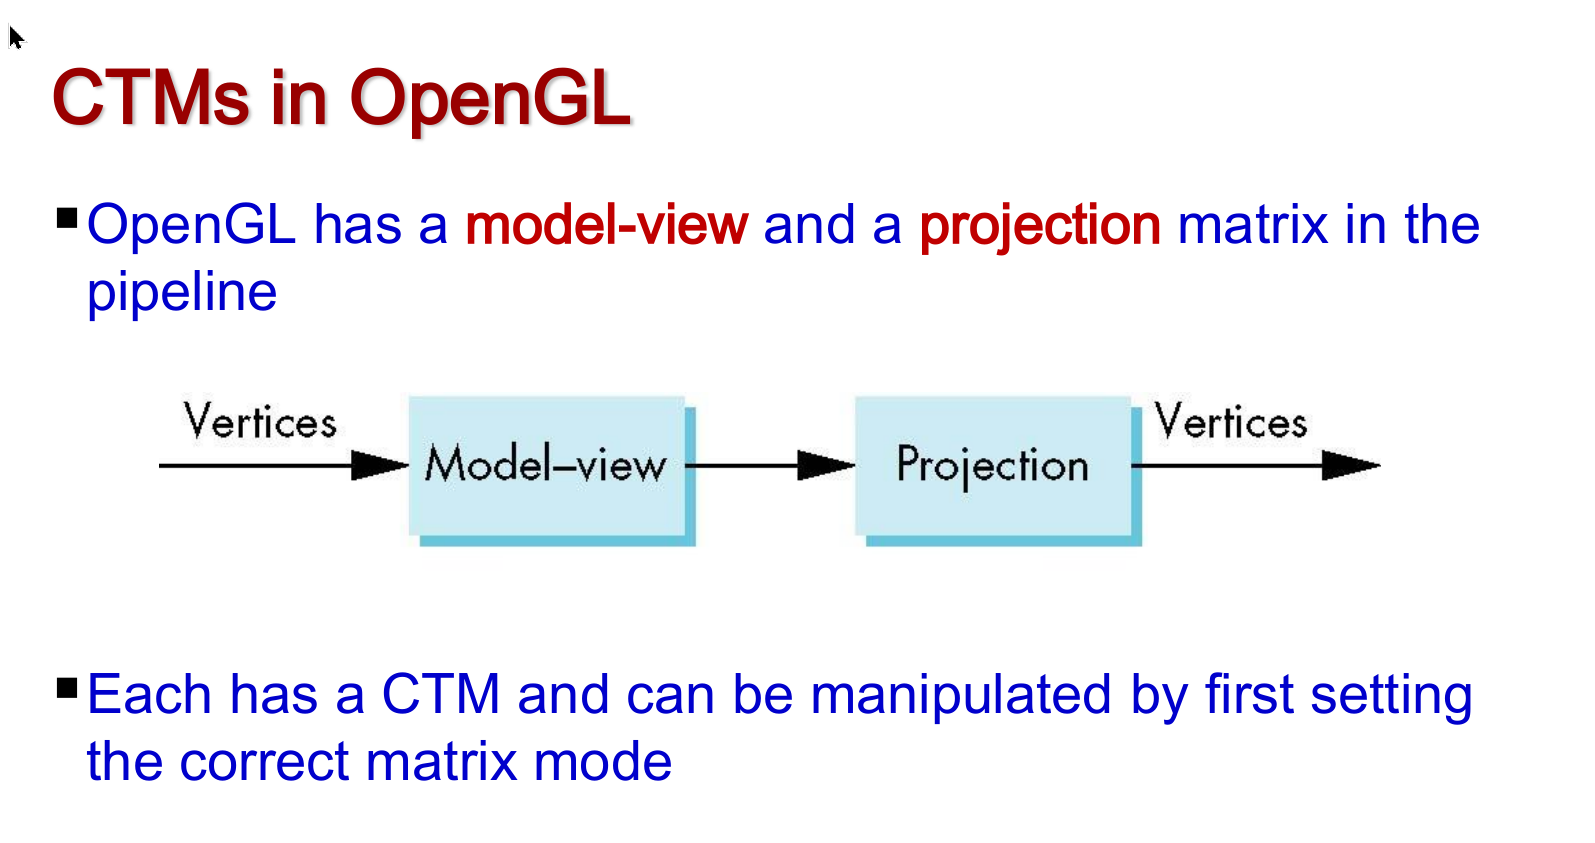
\includegraphics[scale=0.3]{ctm_opengl.png}

\end{frame}

\iffalse
\begin{frame}
    \centering
    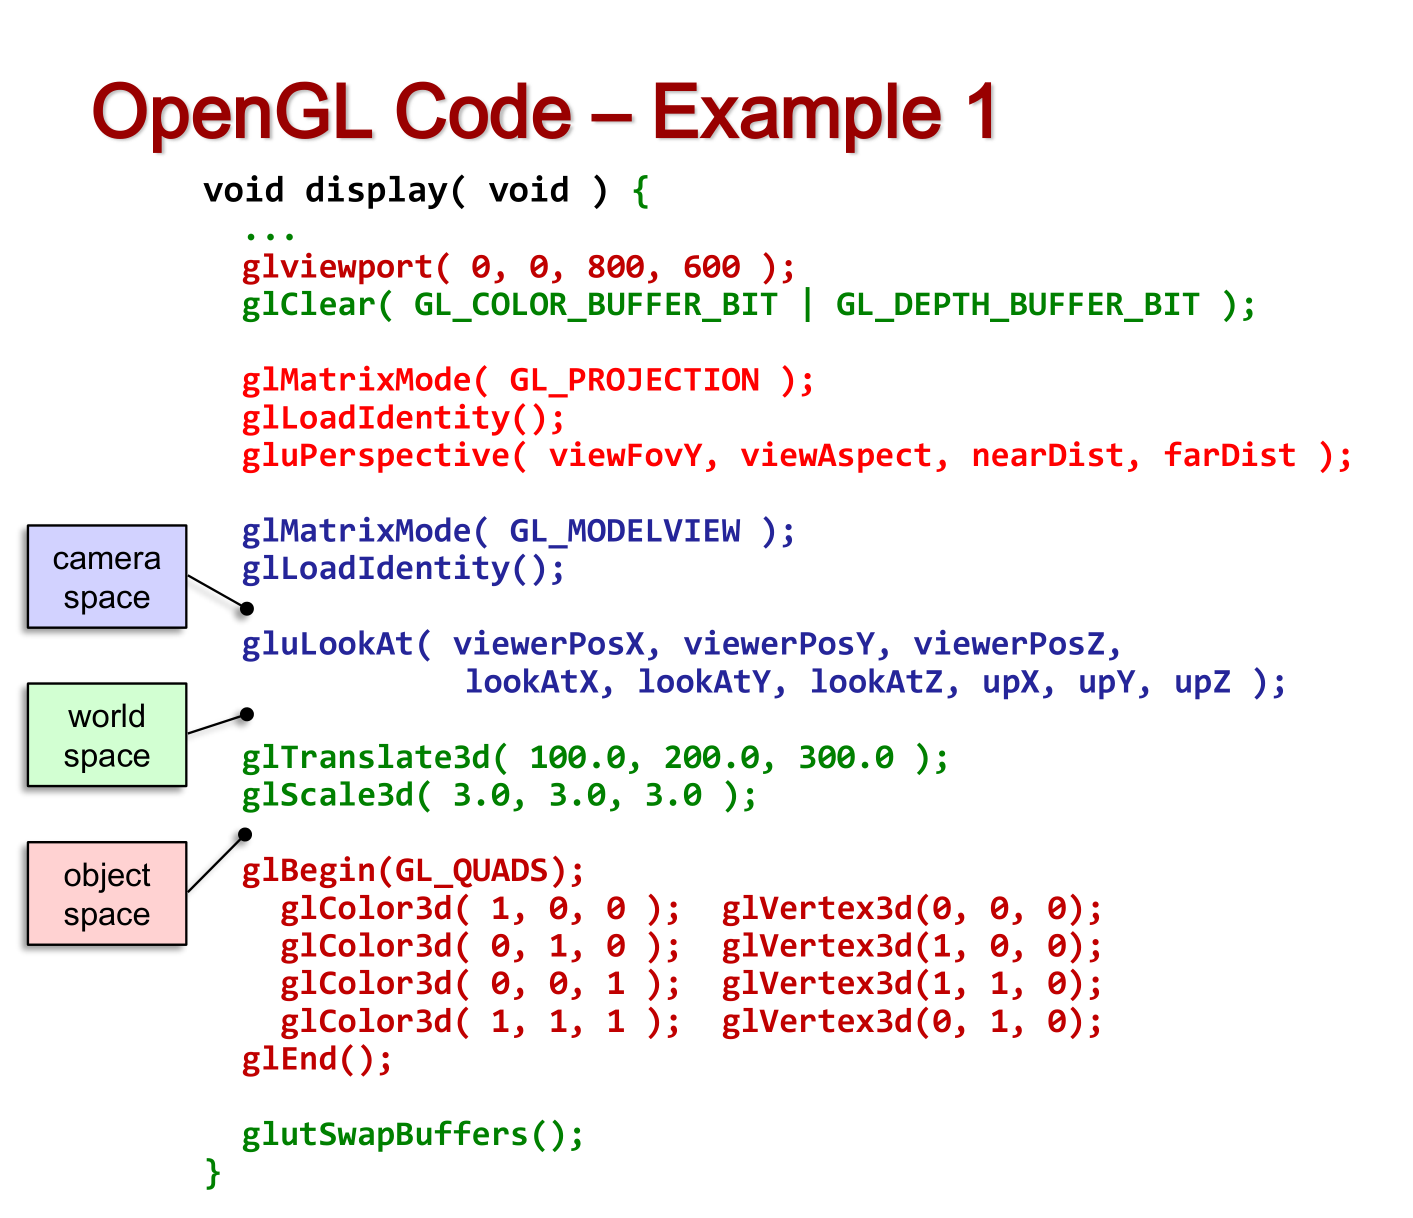
\includegraphics[scale=0.4]{pg48.png}
\end{frame}
\fi

\begin{frame}
    \centering
    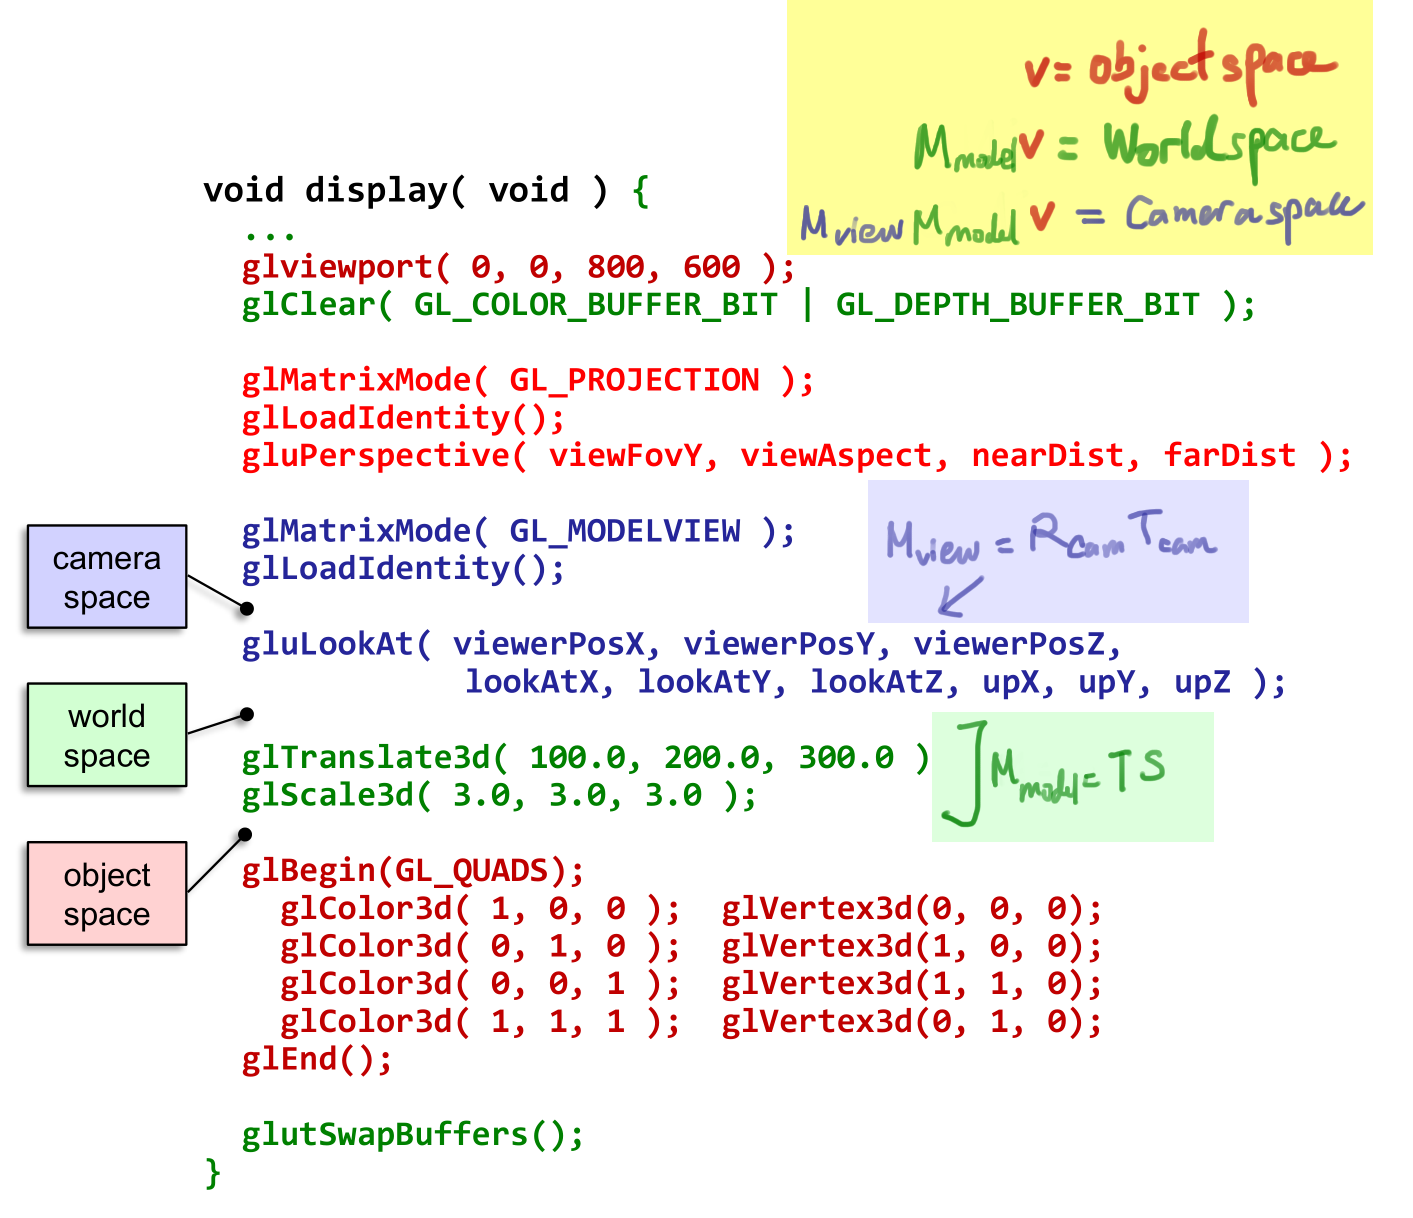
\includegraphics[scale=0.4]{pg48-annot.png}
\end{frame}

\iffalse
\begin{frame}
    \centering
    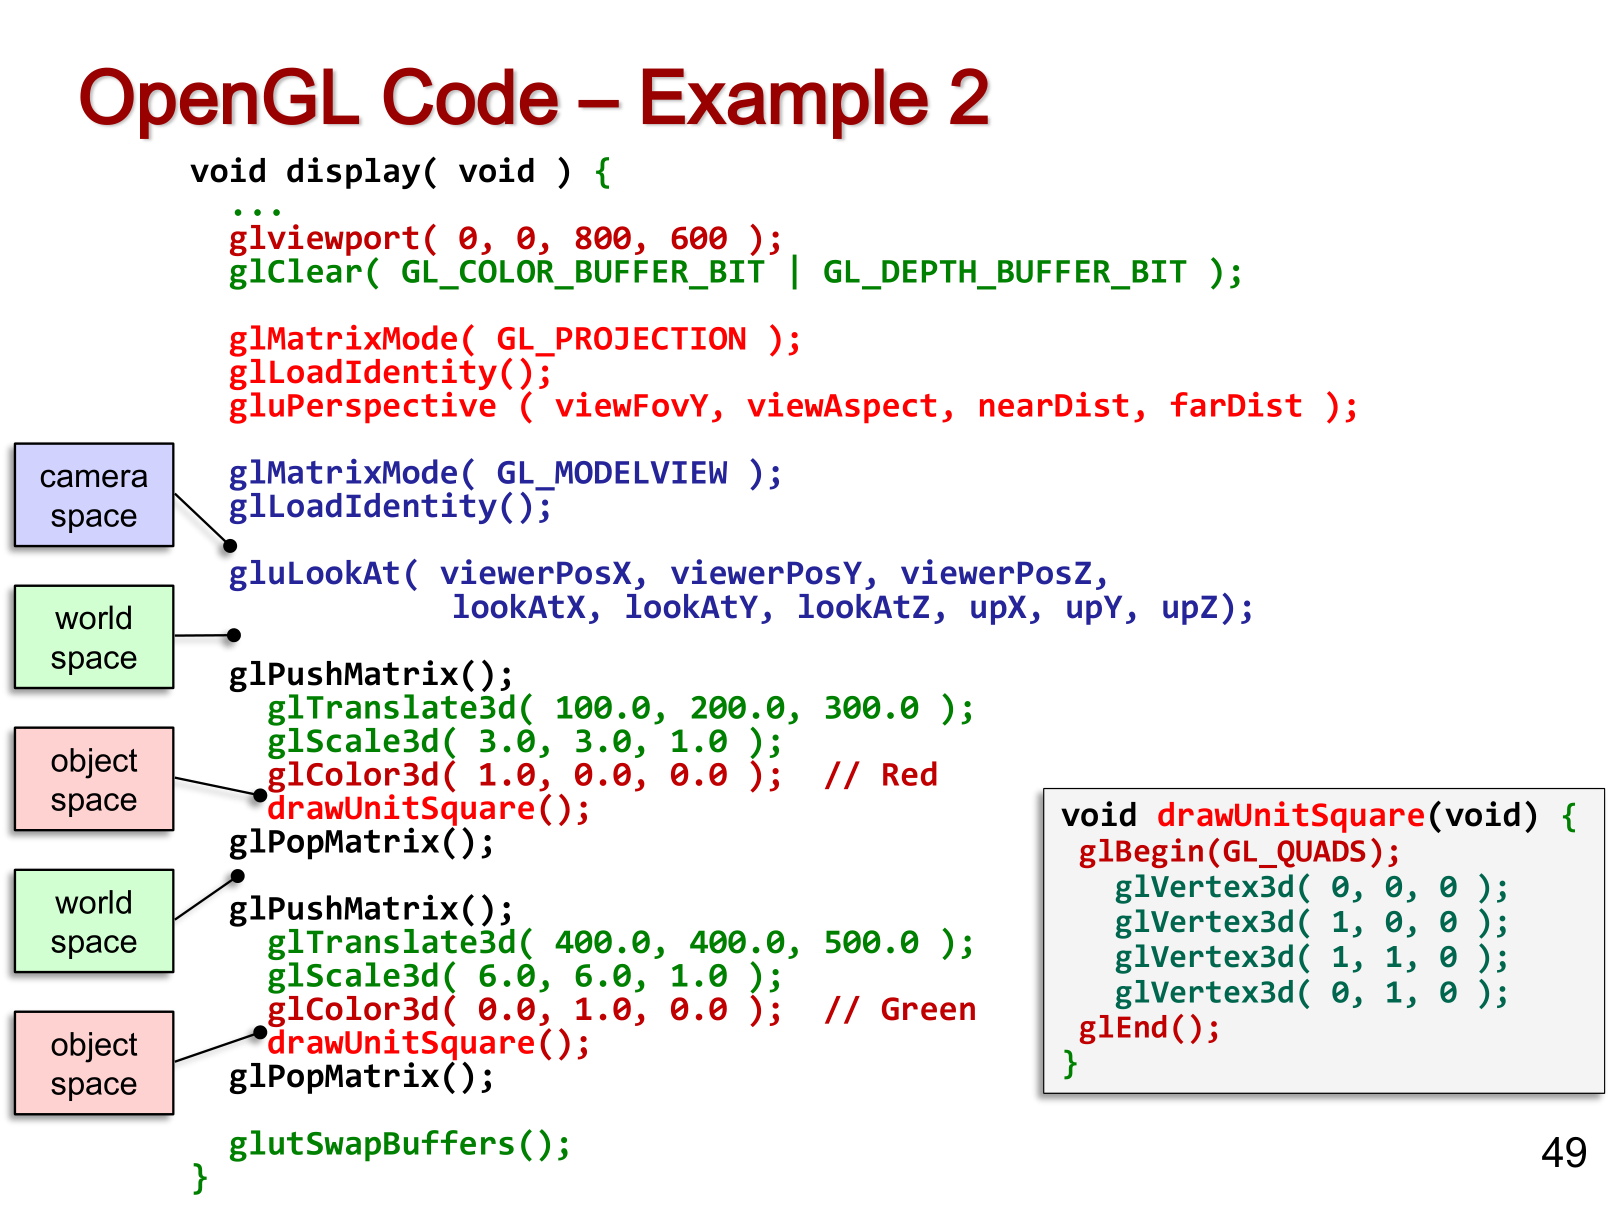
\includegraphics[scale=0.4]{pg49.png}
\end{frame}
\fi

\begin{frame}
    \centering
    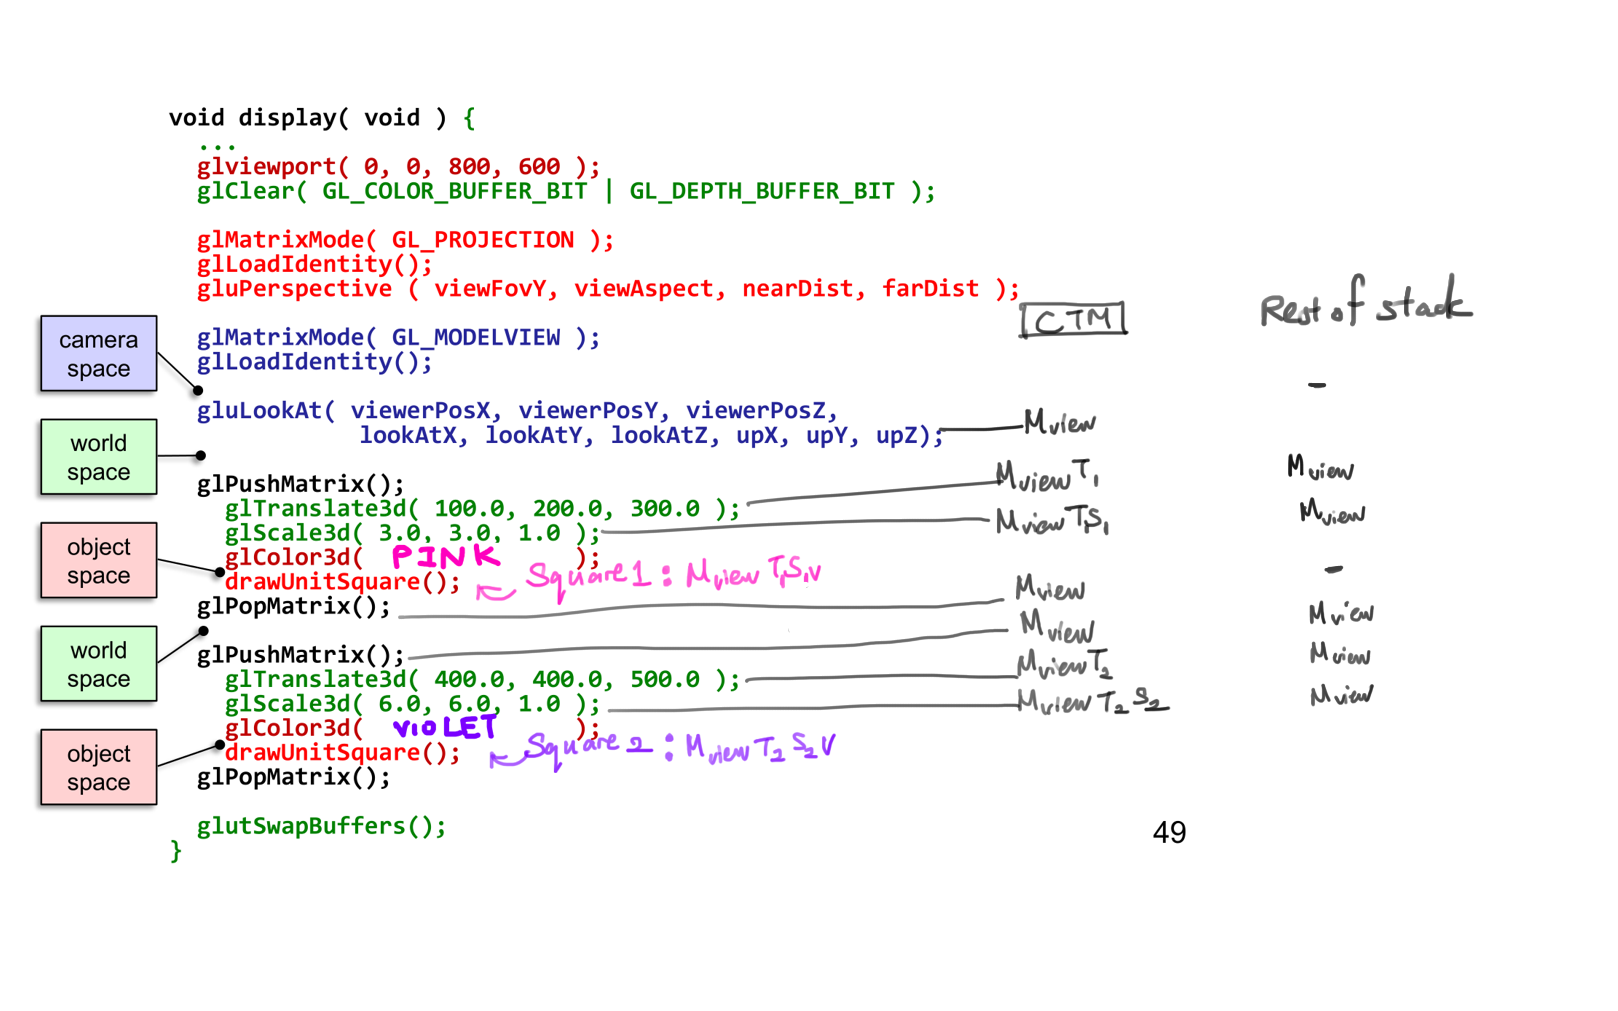
\includegraphics[scale=0.4]{pg49-annot.png}
\end{frame}

\begin{frame}[plain,standout]
    \AlegreyaExtraBold \LARGE
    Tutorial
\end{frame}

\section{Question 1}

\begin{frame}
    \frametitle{Question 1a}
    Referring to Lecture 1 Slide 31. If an imaginary image plane is $d$ unit distance in front of the pinhole camera, 
    what are the coordinates of the projection (on the imaginary image plane) of the 3D point (x, y, z)? 

    \vspace{1em}

    \begin{center}
        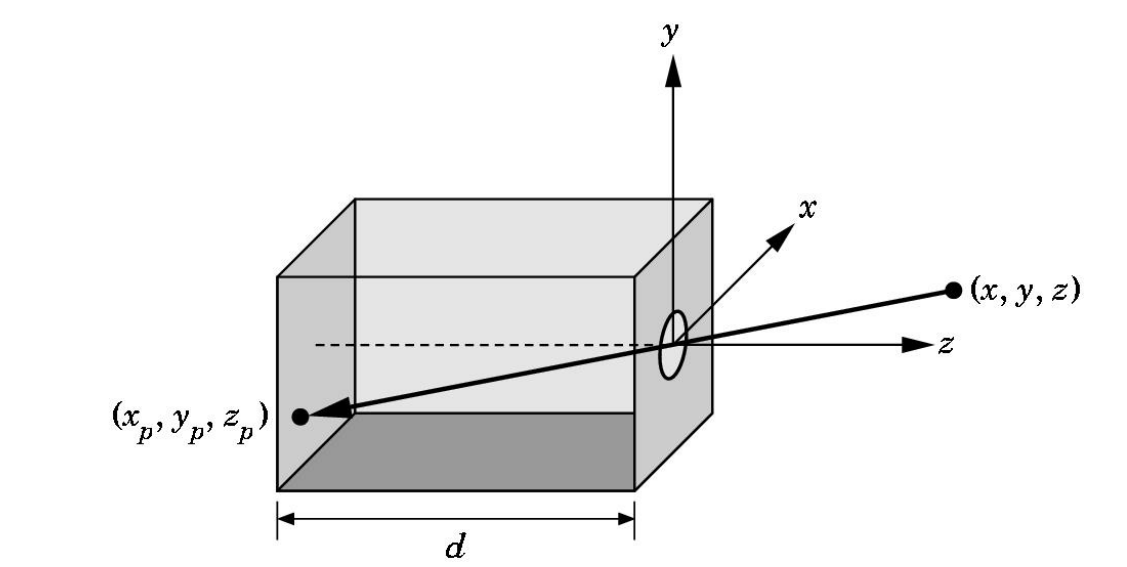
\includegraphics[scale=0.5]{q1-pinhole.png}
    \end{center}
\end{frame}

\begin{frame}
    \frametitle{Question 1a}

    \begin{center}
        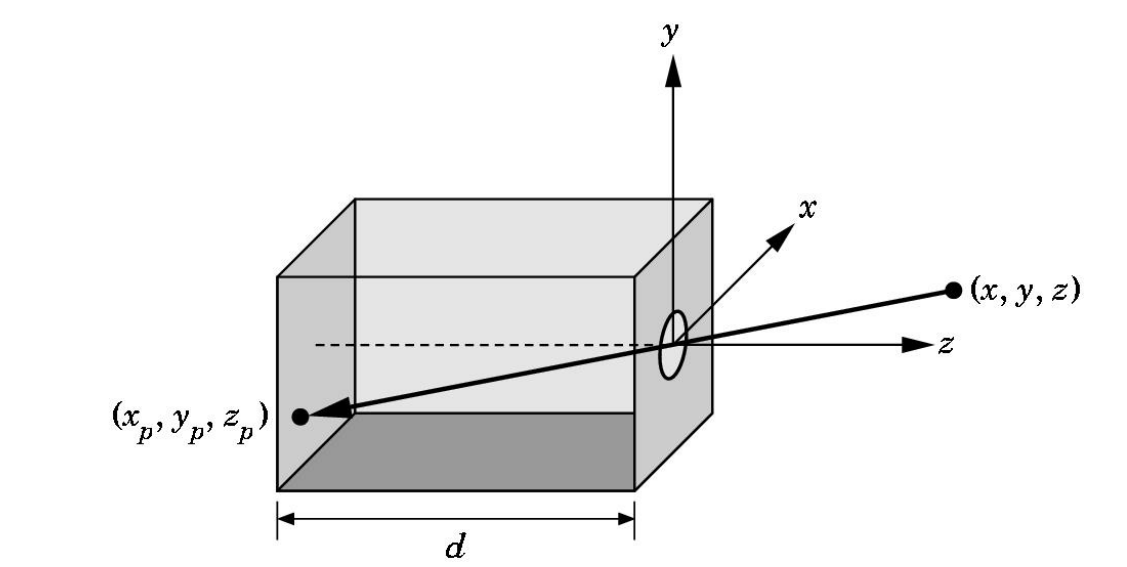
\includegraphics[scale=0.5]{q1-pinhole.png}
    \end{center}
    
    \vspace{1em}

    \begin{tcolorbox}
        \centering
        $\frac{x}{x'} = \frac{y}{y'} = \frac{z}{z'} \text{ and by definition } z' = d$
        $ x' = \frac{dx}{z} \quad y' = \frac{dy}{z} \quad z' = d$
    \end{tcolorbox}

\end{frame}

\begin{frame}
    \frametitle{Question 1b}
    In the above setup, the camera's center of projection is conveniently located at the origin of the “world” coordinate frame, 
    and pointed in the z direction. If the camera's center of projection is not located at the origin, and the camera is pointed in an 
    arbitrary direction, the calculation of the projection becomes very messy. How would you make it less messy?
\end{frame}

\begin{frame}
    \frametitle{Question 1b}

    Reorient the world \textbf{with respect to the camera's rotation and translation}.

    \vspace{1em}

    Visualization: \url{https://imgur.com/a/sXuYgaM}
    
\end{frame}

\begin{frame}
    \frametitle{Explanation}

    \begin{center}
        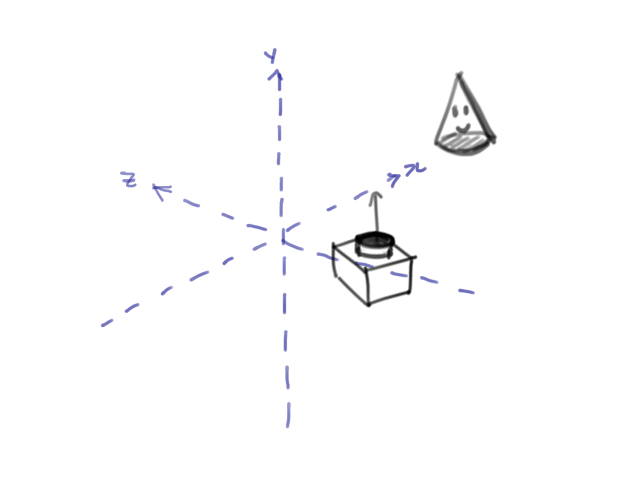
\includegraphics[]{q1b-orig.png}
    \end{center}

    \small
    \begin{itemize}
        \item \textcolor{orange}{Camera axes} and \textcolor{blue}{world axes} are not not equivalent
        \item The cone is represented in \textcolor{blue}{world axes}.
        \item We undo the transformation by \textbf{translating everything by the camera's distance from the origin},
        \item and then \textbf{rotating everything by the camera's rotation}.
        \item And now the \textcolor{orange}{camera axes} and \textcolor{blue}{world axes} are aligned.
    \end{itemize}

\end{frame}

\section{Question 2}

\begin{frame}
    \frametitle{Question 2}

    Why do we want to perform view transformation?
\end{frame}

\begin{frame}
    \frametitle{See Q1b}

    \begin{center}
        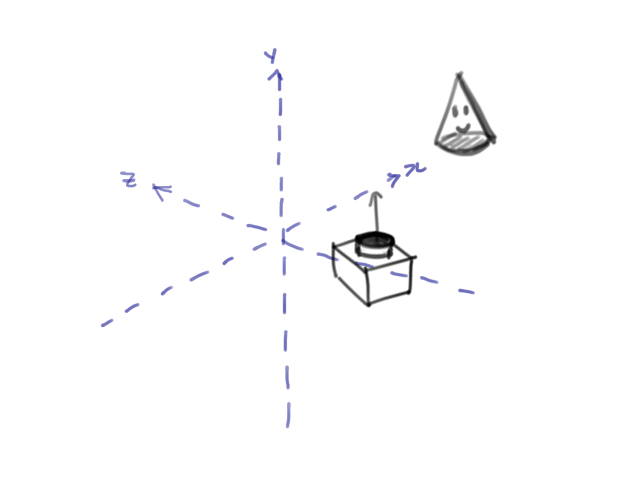
\includegraphics[scale=1.3]{q1b-orig.png}
    \end{center}

\end{frame}

\begin{frame}
    \frametitle{See Q1b}

    \begin{center}
        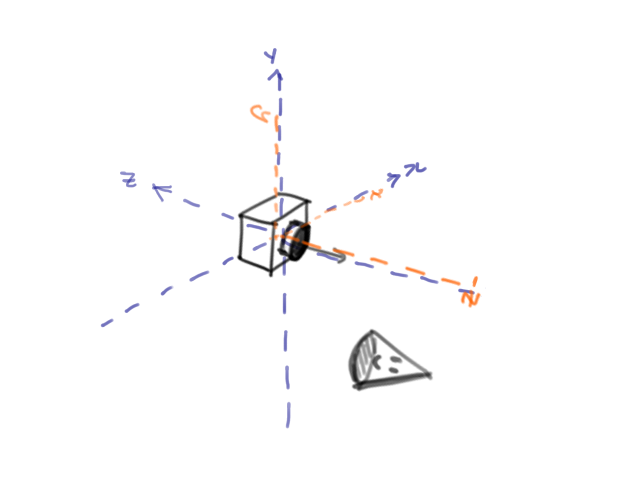
\includegraphics[scale=1.3]{q1b-align.png}
    \end{center}

\end{frame}

\section{Question 3}

\begin{frame}
    \frametitle{Question 3}
    Explain the purpose of the “up-vector” provided to the \texttt{gluLookAt()} function. 
\end{frame}

\begin{frame}
    \frametitle{To prevent the camera from 'rolling'}

    \begin{center}
        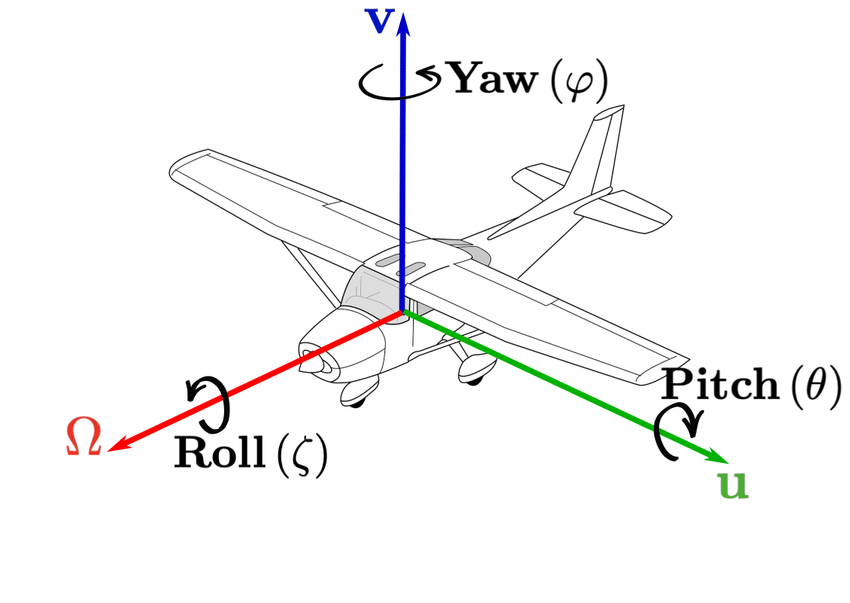
\includegraphics[scale=0.3]{yaw-pitch-roll.png}
    \end{center}

    By defining the "up-vector  we establish a vertical plane for the $y$ and $z$ axes of the camera coordinates.
\end{frame}

\begin{frame}
    \frametitle{Question 3b}

    Why does the “up-vector” not need to be perpendicular to the view direction?

\end{frame}

\begin{frame}
    \frametitle{We can derive our 3 axes as such:}

    \begin{center}
        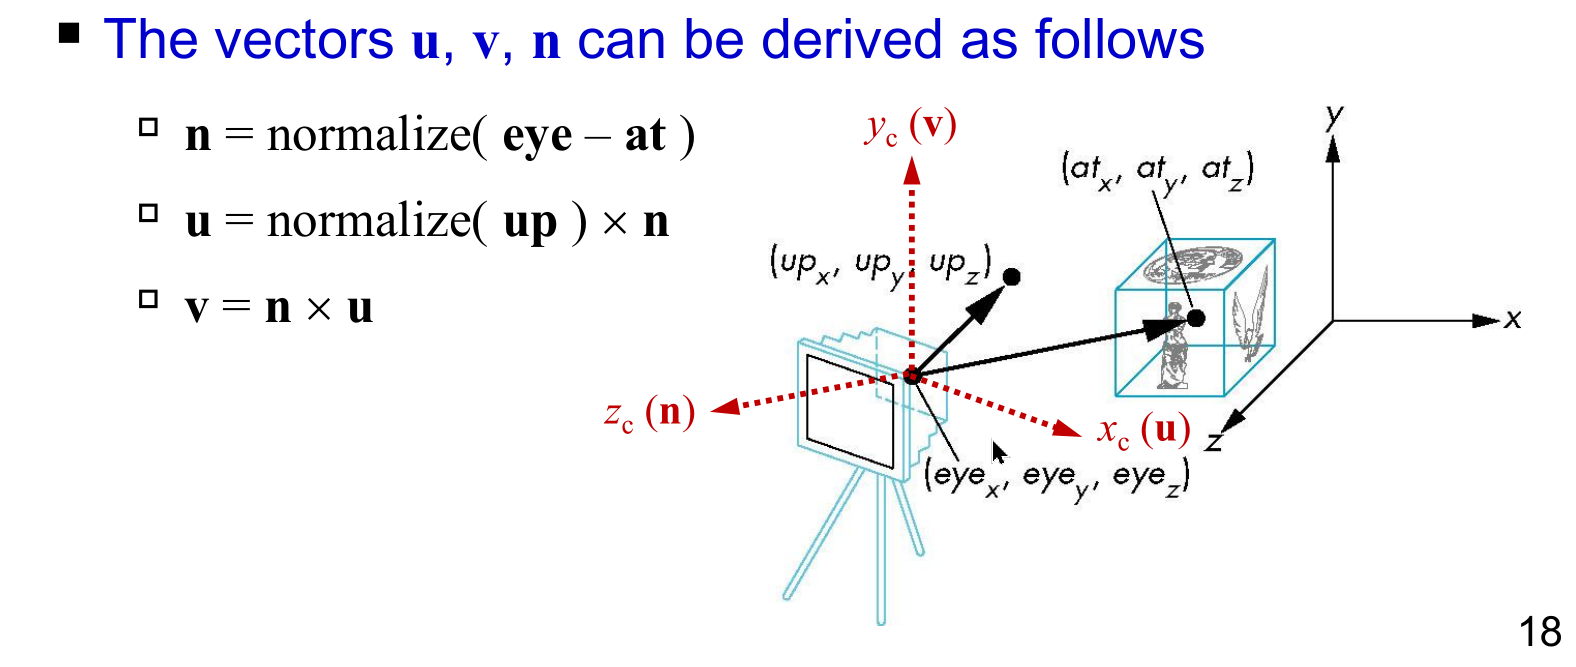
\includegraphics[scale=0.3]{glulookat.png}
    \end{center}

    \begin{tcolorbox}
        As long as the up-vector is \textbf{not parallel} to the view direction and 
        \textbf{is not zero vector}, it already \textcolor{teal}{uniquely defines the y-axis} of the camera.
    \end{tcolorbox}

\end{frame}

\begin{frame}
    \frametitle{We can derive our 3 axes as such:}

    \begin{center}
        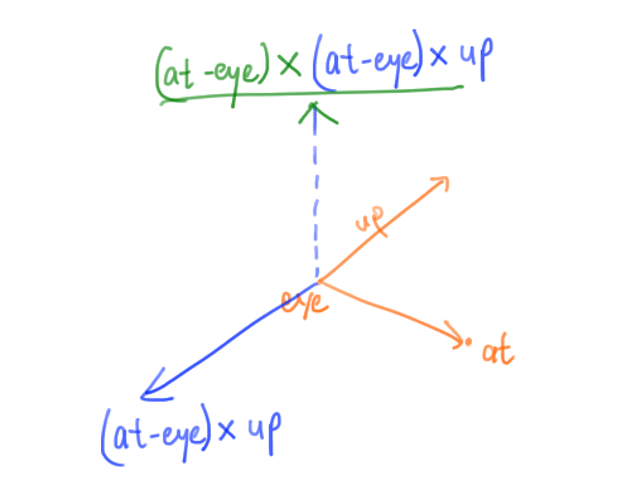
\includegraphics[scale=1.3]{q3.png}
    \end{center}

\end{frame}

\iffalse
\begin{frame}
    \frametitle{Default \texttt{gluLookAt} values}
    
    eye = $(0, 0, -1)$\\
    at = $(0, 0, 0)$\\
    up = $(0, 1, 0)$\\

\end{frame}
\fi

\section{Question 4}

\begin{frame}
    \frametitle{Question 4}
    Replace the following \texttt{gluLookAt()} function call with one or more calls to 
    \texttt{glRotated()} and \texttt{glTranslated()}.

    When using \texttt{glRotated()}, you are allowed to rotate about the x-axis, 
    y-axis and z-axis only.

    \vspace{1em}

    \begin{tcolorbox}[colback=violet!5!white]
        \centering
        \texttt{gluLookAt( ex, ey, ez, ex, ey, ez+1, 0, -1, 0 );}
    \end{tcolorbox}
\end{frame}

\begin{frame}
    \frametitle{Analysis of \texttt{gluLookAt}}

    eye = $(e_x, e_y, e_z)$\\
    at = $(e_x, e_y, e_z+1)$\\
    eye - at = $(0, 0, -1)$\\
    up = $(0, -1, 0)$\\

    \vspace{1em}

    \begin{tcolorbox}
        $z$ axis: $n$ = eye - at = $(0, 0, -1)$\\
        $x$ axis: $u$ = $\|up\| \times \|n\| = (1, 0, 0)$\\
        $y$ axis: $v$ = $\|n\| \times \|u\| = (0, 0, -1) \times (1, 0, 0) = (0, -1, 0)$\\
        camera position = $(e_x, e_y, e_z)$\\
    \end{tcolorbox}

\end{frame}

\begin{frame}

    \begin{center}
        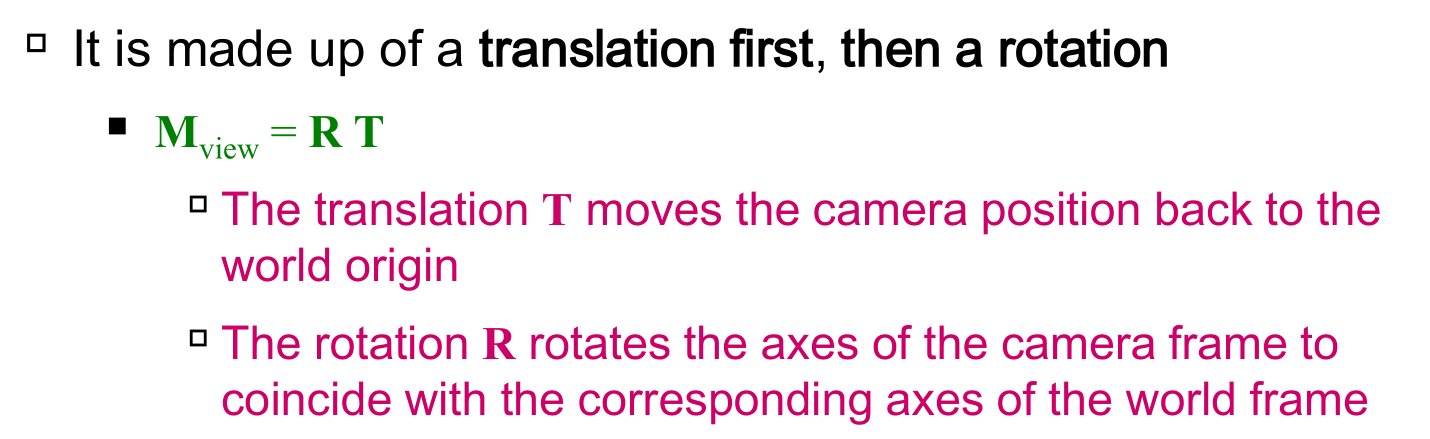
\includegraphics[scale=0.3]{mview.png}
    \end{center}

    \begin{enumerate}
        \item Translate the world towards camera: \textcolor{teal}{\texttt{glTranslate(-ex, -ey, -ez)};}
        \item Rotate the world to align with camera: 
        \begin{itemize}
            \item Notice that the camera z and y coordinates are flipped $z_c = n = -(0,0,1)$ and $y_c = v = -(0,1,0)$
            \item \textcolor{teal}{\texttt{glRotated(180, 1, 0, 0)}}
            \item \textcolor{cyan}{\texttt{glRotated(180, 0, 1, 0); glRotated(180, 0, 0, 1);}}
        \end{itemize}
    \end{enumerate}

\end{frame}

\section{Question 5}

\begin{frame}
    \frametitle{Question 5}
    A vertex, whose camera coordinates are (4, 6, -6), is being projected using the following OpenGL orthographic projection:

    \vspace{1em}

    \begin{tcolorbox}[colback=violet!5!white]
        \centering
        \texttt{glOrtho( -10, 10, -10, 10, 0, 8 );}
    \end{tcolorbox}

    \vspace{1em}

    What will be the vertex's Normalized Device Coordinates (NDC)?
\end{frame}

\begin{frame}
    \frametitle{Coordinates through pipeline}

    \begin{center}
        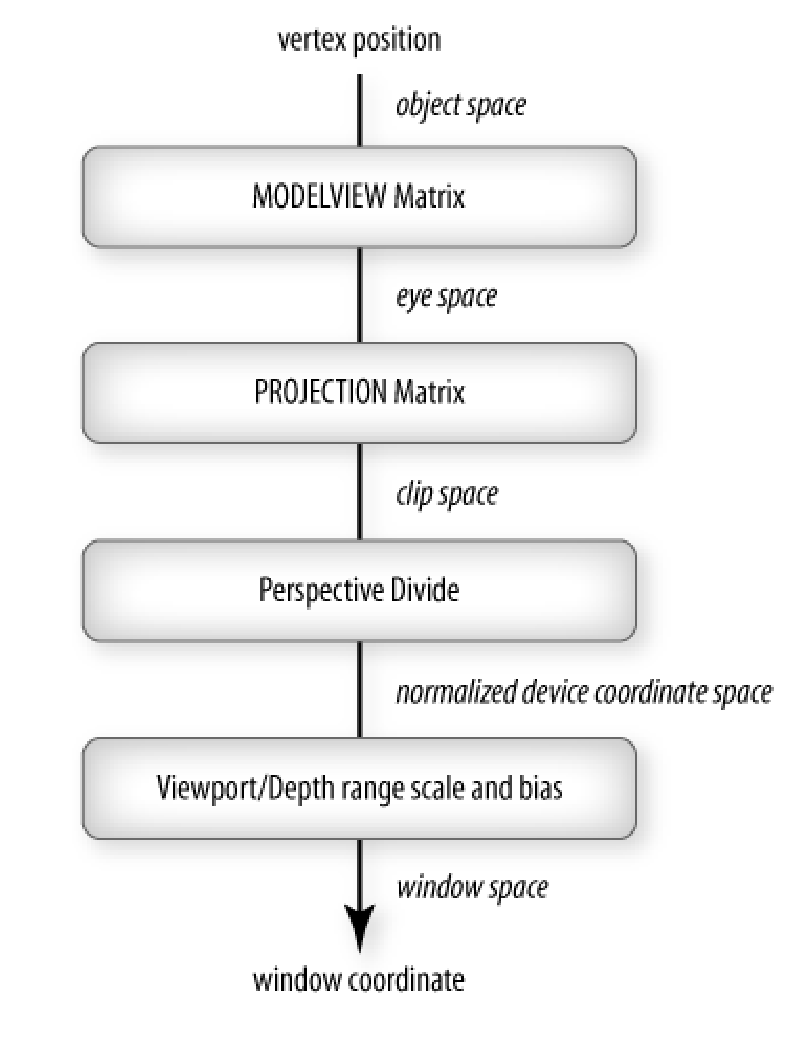
\includegraphics[scale=0.3]{coordinate_pipeline.png}
    \end{center}

    Camera coordinates to NDC space: 
    \begin{enumerate}
        \item If vertex is within the clipping region, it is mapped in NDC space
        \item NDC space is scaled to a \textbf{$2 \times 2 \times 2$ volume}
    \end{enumerate}

\end{frame}

\begin{frame}
    \frametitle{Orthographic projection}

    \begin{center}
        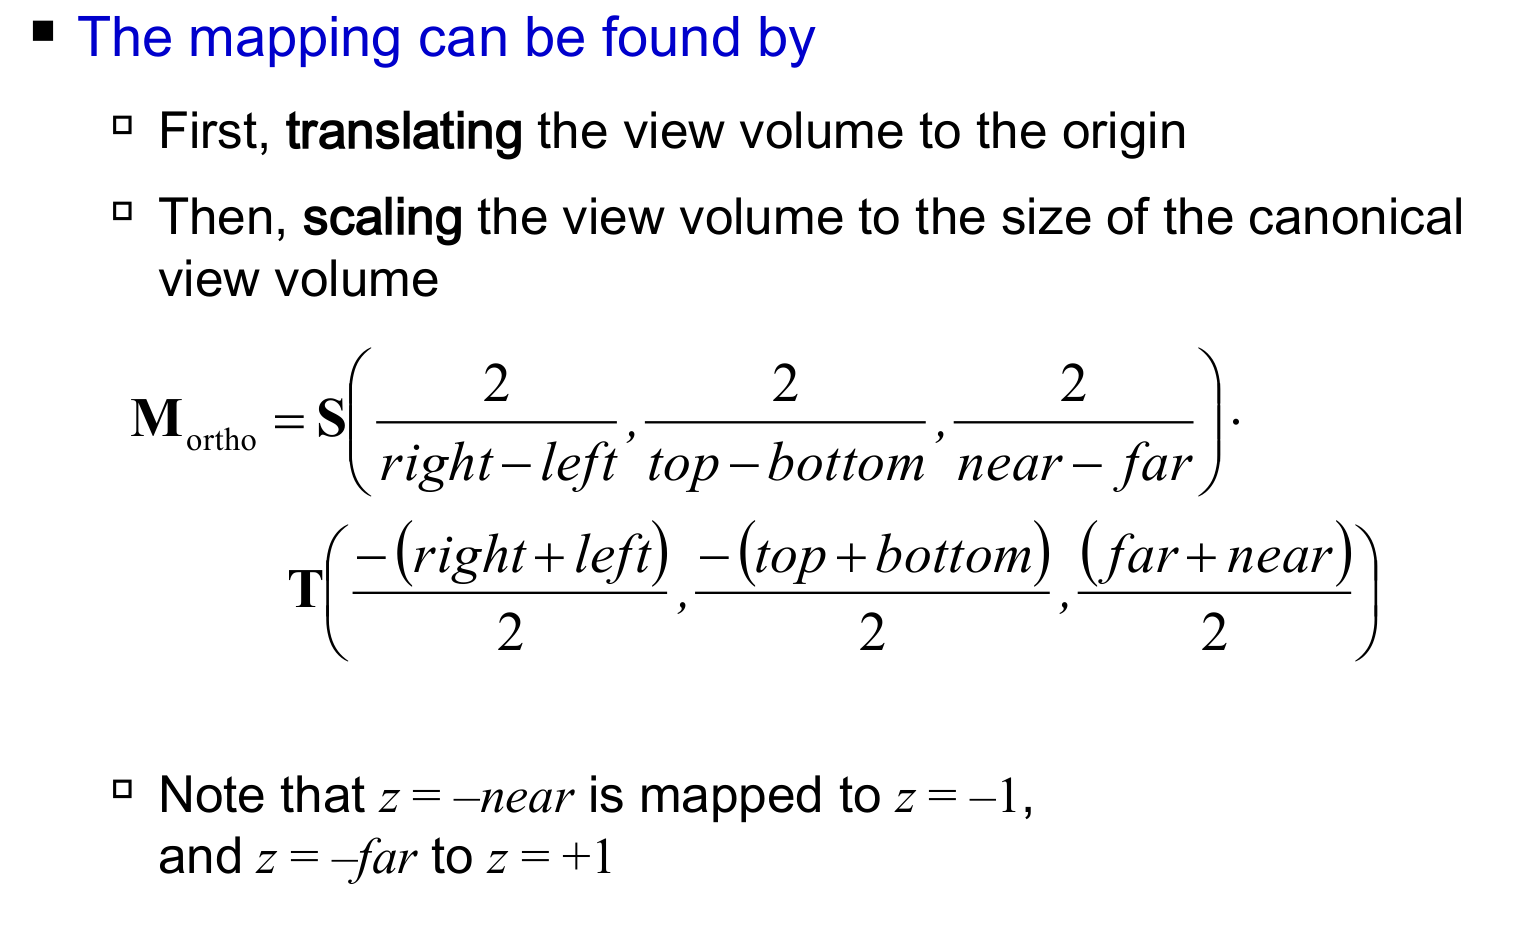
\includegraphics[scale=0.3]{ortho-proj.png}
    \end{center}

\end{frame}

\begin{frame}
    \frametitle{Orthographic projection}

    \begin{tcolorbox}[colback=violet!5!white]
        \begin{center}
            \texttt{glOrtho( l, r, b, t, n, f );}
        \end{center}
    \end{tcolorbox}

    \begin{eqnarray*}
        \mathbf{T} &=& T(\frac{-(10-10)}{2} , \frac{-(10-10)}{2} , \frac{8+0}{2})\\
        &=& T(0,0,4)\\
        \mathbf{S} &=& S(\frac{2}{10 - (-10)} ,\frac{2}{10 - (-10)}, \frac{2}{0 - 8} )\\
        &=& S(0.1,0.1,-0.25)\\
        \mathbf{M}v &=& \mathbf{ST} (4,6,-6)\\
        &=& \mathbf{S} (4,6,-2)\\
        &=& (0.4,0.6,0.5)\\
    \end{eqnarray*}

\end{frame}

\section{Question 6}

\begin{frame}
    \frametitle{Question 6}
    A rectangle has vertices A: (6, -4, -10), B: (14, -4, -10), 
    C: (14, 8, -10), D: (6, 8, -10) in the camera space. 

    \vspace{1em}

    Write a \texttt{glFrustum} function call to set up a view frustum that 
    will maximize the image size of the rectangle, and the entire 
    rectangle must appear in the image. The near and far plane 
    distances should be set as 5 and 15 respectively. 
\end{frame}

\begin{frame}

    \begin{center}
        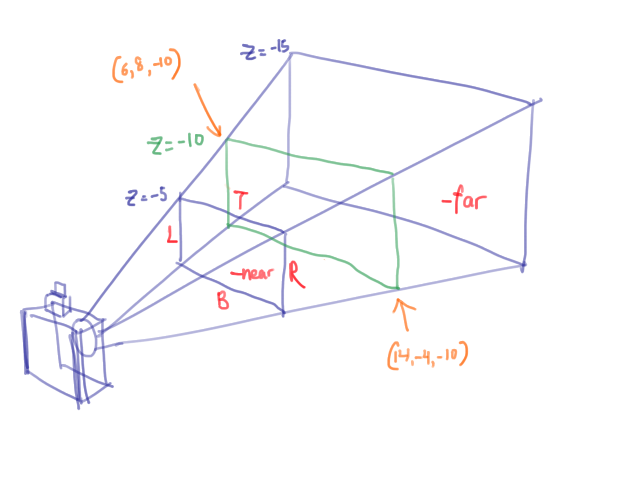
\includegraphics[scale=1.2]{glFrustum-demo.png}
    \end{center}

    \begin{tcolorbox}[colback=violet!5!white]
        \begin{center}
            \texttt{glOrtho( 3, 7, -2, 4, 5, 15);}
        \end{center}
    \end{tcolorbox}

\end{frame}

\section{Question 7}

\begin{frame}
    \frametitle{Question 7}
    A viewpoint at (vx, vy, vz) is looking at the center (cx, cy, cz) 
    of a sphere of radius R. Complete the following OpenGL program to 
    set up a view transformation and an orthographic projection 
    so that the entire sphere appears as big as possible in a 
    square viewport.

    \vspace{1em}

    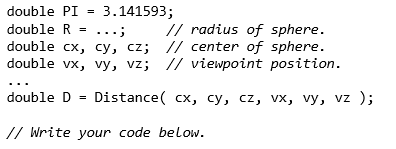
\includegraphics[]{q7-qn.png}
    

\end{frame}

\iffalse
\begin{frame}
    \frametitle{Question 7}
    You should specify the tightest near and far planes. 
    Assume that the up-vector of the camera is always (0, 1, 0) 
    (in the world space), and the viewpoint is always outside the sphere. 
    You must use the functions gluLookAt() and glOrtho(). 
    The distance between (cx, cy, cz) and (vx, vy, vz) is already computed as D.

    \vspace{1em}

    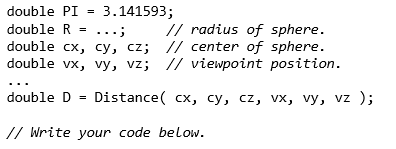
\includegraphics[]{q7-qn.png}

\end{frame}
\fi

\begin{frame}
    \frametitle{Code}
    
    \begin{center}
        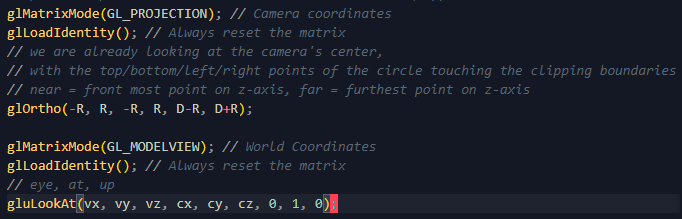
\includegraphics[scale=0.8]{q7-ans.png}
    \end{center}

\end{frame}

\section{Question 8}

\begin{frame}
    \frametitle{Question 8}
    Re-implement the \texttt{gluPerspective()} function by using the 
    \texttt{glFrustum()} function. You can make use of the tangent function 
    \texttt{tan()}, which takes an angle parameter (in radians). 

    \begin{tcolorbox}
        \small
        \texttt{void gluPerspective(\\
            \tab \tab double fovy, double aspect, \\
            \tab \tab double near, double far) \{ \\
            \tab const double PI = 3.141592;\\
        \}}
    \end{tcolorbox}
\end{frame}

\begin{frame}
    \frametitle{Question 8}

    \begin{center}
        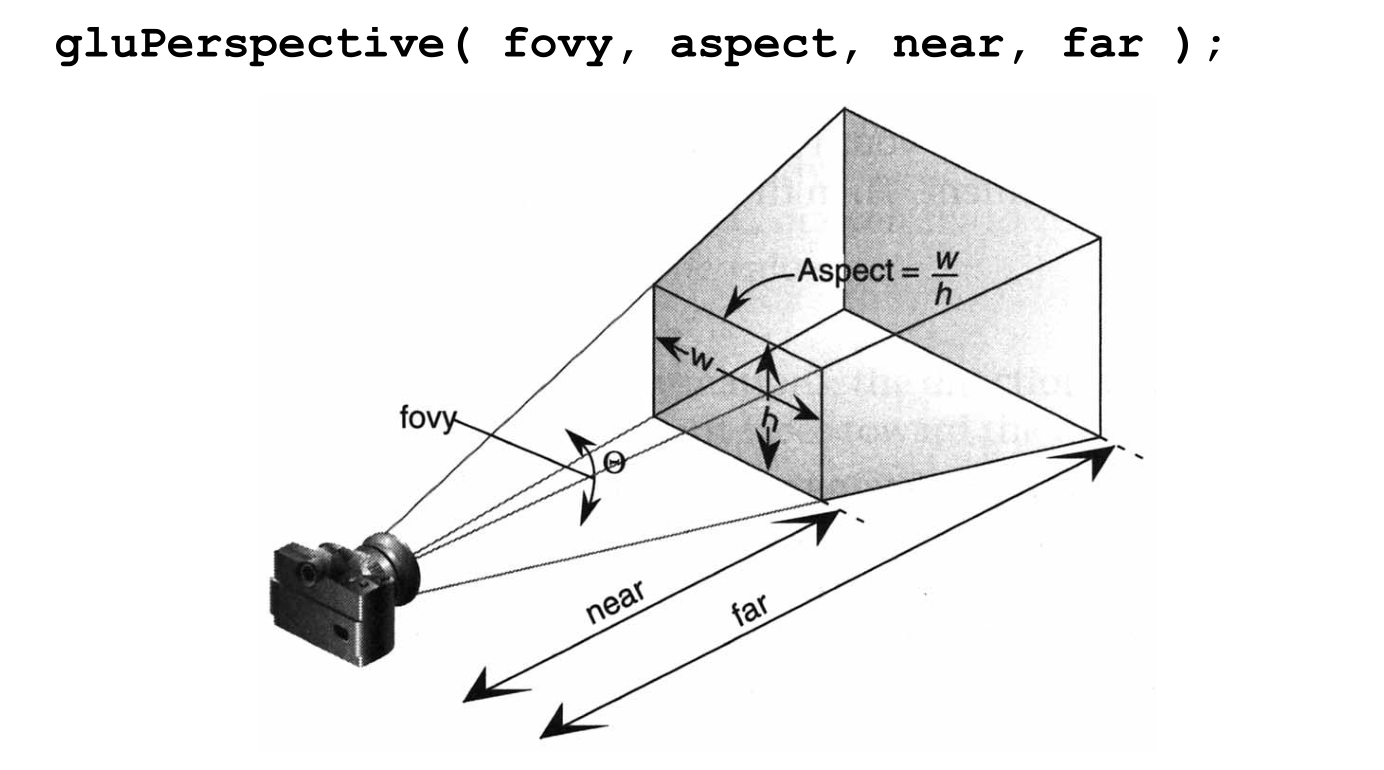
\includegraphics[scale=0.3]{gluPerspective.png}
    \end{center}

    left = $-\frac{h}{2}$, right = $\frac{h}{2}$, bottom = $-\frac{w}{2}$, top = $\frac{w}{2}$.\\

\end{frame}

\begin{frame}
    \frametitle{}
    Let aspect ratio be $a = \frac{w}{h}$.\\
    Let fovy be $\theta$.\\

    \vspace{1em}

    By trigonometry, $h = 2\tan(\frac{\theta}{2}) \times \text{near}$.\\
    By definition, $w = ah$.

    \vspace{1em}

    \begin{center}
        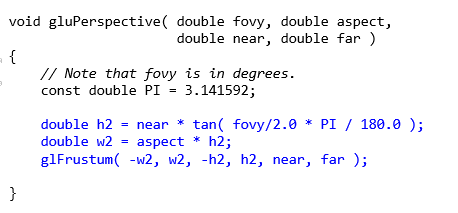
\includegraphics[scale=0.8]{q8-ans.png}
    \end{center}

\end{frame}

\section{Question 9}

\iffalse
\begin{frame}
    \frametitle{Question 9 [Optional]}
    Prove that OpenGL perspective transformation preserves the depth 
    order of any two points on the same projector and in the 
    view volume. (Quite tedious)
\end{frame}
\fi

\begin{frame}[plain,standout]
    \AlegreyaExtraBold \LARGE
    Attendance taking
\end{frame}

\ThankYou
\begin{frame}[plain,standout]
    Thanks! Get the slides here after the tutorial.\\
    \vspace{2em}
    \scalebox{3}{\faGithub}\par\bigskip
    \url{https://trxe.github.io/cs3241-notes}
\end{frame}

\end{document}